\documentclass[12pt, twoside]{article}
\setlength{\headheight}{14.49998pt}
\usepackage{xeCJK}

% Pseudo-code
\usepackage{algorithm}
\usepackage{algpseudocode}

% Wrap-figure
\usepackage{wrapfig}

\usepackage{listings}
\usepackage{lstautogobble} % Fix relative indenting
\usepackage{xcolor}
\usepackage{multirow}

\usepackage[a4paper, left=3.17cm, right=3.17cm, top=2.54cm, bottom=2.54cm]{geometry}
\usepackage{fancyhdr} % header and footer
\usepackage[T1]{fontenc}
\usepackage{mathptmx}
\usepackage{amsmath}
\usepackage{amsfonts}
\usepackage{chemformula}
\usepackage{cite}
\usepackage[colorlinks, linkcolor=black, anchorcolor=black, citecolor=black]{hyperref}
\usepackage{graphicx}
\usepackage{hyperref}

\setCJKmainfont{Songti SC}
\setCJKmonofont{Songti SC}

% Define colors for code listing
\definecolor{bluekeywords}{rgb}{0.13,0.13,1}
\definecolor{greencomments}{rgb}{0,0.5,0}
\definecolor{redstrings}{rgb}{0.9,0,0}
\definecolor{graynumbers}{rgb}{0.5,0.5,0.5}

\lstset{
  autogobble,
  columns=fullflexible,
  showspaces=false,
  showtabs=false,
  breaklines=true,
  showstringspaces=false,
  breakatwhitespace=true,
  escapeinside={(*@}{@*)},
  commentstyle=\color{greencomments},
  keywordstyle=\color{bluekeywords},
  stringstyle=\color{redstrings},
  numberstyle=\color{graynumbers},
  basicstyle=\ttfamily\footnotesize,
  frame=l,
  framesep=12pt,
  xleftmargin=12pt,
  tabsize=4,
  captionpos=b
  language=C++
  % backgroundcolor=\color{black!5},
}

% c syntex shortcut
\newcommand\codestyle{\lstset{
  autogobble,
  columns=fullflexible,
  showspaces=false,
  showtabs=false,
  breaklines=true,
  showstringspaces=false,
  breakatwhitespace=true,
  escapeinside={(*@}{@*)},
  commentstyle=\color{greencomments},
  keywordstyle=\color{bluekeywords},
  stringstyle=\color{redstrings},
  numberstyle=\color{graynumbers},
  basicstyle=\ttfamily\footnotesize,
  frame=l,
  framesep=12pt,
  xleftmargin=12pt,
  tabsize=4,
  captionpos=b
  language=C++
  % backgroundcolor=\color{black!5},
}}

% c environment
\lstnewenvironment{code}[1][]
{
  \codestyle
  \lstset{#1}
}
{}

% c for external files
\newcommand\codeexternal[2][]{{
    \codestyle
    \lstinputlisting[#1]{#2}
}}

% c for inline
\newcommand\codeinline[1]{{\codestyle\lstinline!#1!}}

% End of c syntex highlight configuation.

% show paragraphs in table of contentes
\setcounter{tocdepth}{4}
\setcounter{secnumdepth}{4}

\graphicspath{{figures/}}

\setlength{\parskip}{0.5em}
\title{内存分配实验}
\author{\textup{吴清柳}}
\begin{document}
\begin{titlepage}
	\newcommand{\HRule}{\rule{\linewidth}{0.5mm}}
	
\includegraphics[width=8cm]{title/logo_bupt.png}\\[1cm]
	\center
	\quad\\[1.5cm]
	\textsl{\Large 北京邮电大学}\\[0.5cm]
	\textsl{\large  计算机学院}\\[0.5cm]
	\makeatletter
	\HRule \\[0.4cm]
	{\huge \bfseries \@title}\\[0.4cm]
	\HRule \\[0.5cm]
	\begin{minipage}{0.4\textwidth}
		% \begin{flushleft} \large
		% 	\emph{Author:}\\
		% 	\@author
		% \end{flushleft}
	\end{minipage}
	\large {(分别使用c++和Rust实现)}\\[2cm]
	~\\[2cm] % Tips: if use previous line, comment or delete this line

	\makeatother
	{\large 姓名: 吴清柳}\\[0.5cm]
	{\large 学号: 2020211597}\\[0.5cm]
	{\large 班级: 2020211323}\\[0.5cm]
	{\large 指导老师: 邵蓥侠}\\[0.5cm]
	{\large \emph{课程名称: 算法设计与分析}}\\[0.5cm]
	{\large \today}\\[2cm]
	\vfill
\end{titlepage}

\tableofcontents
\newpage

% set page stype to fancy then decorate it
\pagestyle{fancy}
\fancyhead{} % clear all header fields
\fancyhead[LE, RO]{吴清柳 2020211597}
\fancyhead[LO, RE]{内存分配实验}
\fancyfoot{} % clear all footer fileds
\fancyfoot[CE, CO]{\thepage}

\section{实验题目}
利用python的json库和csv库,
将Scrapy爬取的保存在json格式中的链家新房数据转为csv格式.\par

\subsection{输入的json格式}
由于Scrapy爬取的数据已经被我做过后处理, 因此看起来比较整洁. 具体格式如下:
\begin{lstlisting}[language=json]
[
    {
        "house_name": "尊悦日坛", // 楼盘名称
        "resblock_type": "商业类", // 类型
        "resblock_location": [ // 地理位置
            "朝阳",
            "朝阳门外",
            "日坛北路19号"
        ],
        "resblock_room": "1室", // 房型
        "resblock_area": "建面 45-135㎡", // 面积
        "house_avg_price": "63000", // 均价
        "house_total_price": "总价350-1200(万/套)" // 总价
    },
    {
        "house_name": "天恒摩墅",
        "resblock_type": "别墅",
        "resblock_location": [
            "房山",
            "房山其它",
            "周口店镇政府东200米"
        ],
        "resblock_room": "3室",
        "resblock_area": "建面 140-160㎡",
        "house_avg_price": "23000",
        "house_total_price": "总价320-530(万/套)"
    },
    
    ...
]
\end{lstlisting}

\subsection{处理过程}
要进行处理的关键步骤罗列如下,
详细实现在data\_process.py中类json2csv中的函数\_data\_process()中:
\begin{itemize}
    \item 去掉字符串字段中的空格, 由于去掉的是前后空格, 使用strip()实现.
    \item 面积和总价所给是一个范围, 将其求\textbf{平均值}并取整. 对于范围的提取和处理,
        使用正则表达式配合对None的判断进行. 正则表达式如下.
        \begin{lstlisting}[language=python]
            # Extract the first one or two integer(s) from string.
            int_re = re.compile(r"^[\D]*(\d+)[\D]*(\d+)?")
        \end{lstlisting}
    \item 对缺失数据, 不进行处理.
\end{itemize}

\paragraph{求平均值的理由} % (fold)
\label{par:求平均值的理由}
相比于最小值和最大值, 平均值更能代表数据的一般特征. 采用面积和总价的最小值的话,
最终得到的统计结果会明显偏小与实际值, 难以合理反应数据分布的影响. 例如,
最小值相同的两份数据A和B, A中可能几乎都是接近最小值的数值,
而B中可能只有寥寥几个数值接近最小值. 使用最小值就难以对此进行表现.\par
因此, 这里采用了对面积和总价求平均的方式.
% paragraph 求平均值的理由 (end)

\subsection{csv数据格式}
对json文件读取并进行上述处理后, 转换到作业所要求的字段名称, 并写入csv文件.
函数为data\_process.py中类json2csv的函数write\_data()中.
csv文件格式如下.
\begin{lstlisting}
名称,类型,行政区,次级地理位置,末级地理位置,房型,面积,总价,均价
尊悦日坛,商业类,朝阳,朝阳门外,日坛北路19号,1室,90,775,63000
天恒摩墅,别墅,房山,房山其它,周口店镇政府东200米,3室,150,425,23000
鲁能·格拉斯小镇,别墅,通州,通州其它,北京市通州区宋庄镇格拉斯小镇营销中心,3室,317,1762,62000

...
\end{lstlisting}

\section{实验过程}
\subsection{归并排序mergesort}
\subsubsection{算法类别}
mergesort(归并排序)是一种基于\textbf{分治}的算法.

\subsubsection{算法思路}
在mergesort中, 待排序数组被分为两等分, 分别排序后合并为一个数组. \par
mergesort是一个递归算法, 持续的将数组二等分并对等分后得到的两个数组
分别进行mergesort, 直到数组不能再分, 此时数组为空或仅剩1个元素.
也就是说, 这是递归的终止情况. 如果数组有多个元素, 将数组分为两等份,
并在每一份上递归的调用mergesort. 最终, 当两半数组都被排序, 对两个数组
执行merge(合并)操作. \par
merge(合并)操作是将两个较小的有序数组结合成一个大的有序数组的过程.

\subsubsection{关键函数及代码段的描述}
采用non-recursive的迭代方式实现mergesort, 基于DRY \footnote{
	DRY: don't repeat yourself, 即不要做重复性的工作,
	通过良好的函数和类的抽象减少冗余和重复代码的出现}
的原则, 将mergesort分为三个函数, 分别是mergeSort(), mergePass(int *x,
int *y, int s, int n)和merge(int *c, int *d, int l, int m, int r). \par
mergeSort()是归并排序的入口函数, 管理步长倍增, 并通过将数组a和数组
b交替作为辅助数组的方式, 减少了一半的元素赋值操作. \par
mergePass()是归并排序中的一遍, 通过不断调用merge(),
将两个子序列用步长s按从小到大的顺序排序. \par
merge()函数将两个子数组c[l, ..., m]和c[m+1, ..., r]合并到d中. \par
函数均使用类似C++的Pseudo-Code描述.
\begin{lstlisting}[language=c++]
/**
 * Iterative mergesort function to sort a[0, ..., n-1], 
 * Merge subarrays in bottam up manner. First merge subarrays of
 * size 1 to create sorted subarrays of size 2, then merge subarrays
 * of size 2 to create sorted subarrays of size 4, and vice versa.
 */
void mergeSort() {
	// Initializing...
	int s = 1;
	while (s < n) {
		// treat b as assistant array
		mergePass(a, b, s, n);
		// double the step size
		s += s;
		// treat a as assistant array
		mergePass(b, a, s, n);
		// double the step size
		s += s;
	}
}

/**
 * A pass of merge with step size of s.
 */
void mergePass(int *x, int *y, int s, int n) {
	int i = 0; // left variable
	// merge until less than 2*s elements left.
	if (i + step_size - 1 < n) {
		// merge till the end of array
	} else {
		// append rest elements of x to y
	}
}

/**
 * Function to merge the two halves c[l, ..., m] and c[m+1, ..., r]
 * to d
 */
void merge(int *c, int *d, int l, int m, int r) {
	int i = l;
	int j = m+1;
	int k = i;
	// merge the two halves of array c to array d
	while(left half not reach the end &&
		right half of c not reach the end) {
			 append smaller element of c[i] and c[j] to d[k]
			 and increase i and k or j and k
		}

	// if left half of array c reaches the end, append rest elements
	// of right half of array c to d
	if (i > m) {
		append rest elements of right half of array c to d
	} else {
		vice versa
	}
}
\end{lstlisting}

\subsubsection{算法时间及空间复杂性分析}
\paragraph{空间复杂度分析}
mergesort需要一个长度为n的辅助数组进行辅助merge, 故空间复杂度为$O(n)$.

\paragraph{时间复杂度分析}
对于mergesort, 比较和挪动元素都发生在merge阶段, 由于对两个元素不进行
比较就不可能进行挪动, 故元素移动次数不会大于比较次数, 只需根据比较次数
即可分析时间复杂度. \par
由于归并排序是递归的过程, 可以方便地写出递推式:
\begin{align}
	C(1)       & = 0                                \nonumber \\
	C_{max}(n) & = 2C(\frac{n}{2}) + n-1            \nonumber \\
	C_{min}(n) & = 2C(\frac{n}{2}) + \frac{n}{2}    \nonumber \\
	C_{avg}(n) & = 2C(\frac{n}{2}) + \frac{3n-2}{2} \nonumber
\end{align}
令\(n=2^k\), 将式中$O(n)$项
用$O(n)$代替, 则最好, 最坏和平均情形都为相同形式, 即
\begin{equation}
	C(n) = 2C(\frac{n}{n})+(n)
\end{equation}
记$C(n)$为比较次数, 有
\begin{gather}
	C'(0) = 0            \nonumber \\
	C'(k) = 2C'(k-1)+2^k \nonumber
\end{gather}
得
\begin{equation}
	C'(k) = 2^kC'(0)+k\cdot 2^k = k\cdot 2^k \nonumber
\end{equation}
即
\begin{equation}
	C(n) = n\log_2{n} \nonumber
\end{equation}
综上, mergesort的时间复杂度为$O(n\log{n})$

\subsection{应用尾递归优化的快速排序quicksort}
\subsubsection{算法类别}
quicksort(快速排序)和mergesort一样, 也是一种\textbf{分治法}算法.

\subsubsection{算法思路}
quicksort将一个元素作为\textbf{pivot(枢轴)}, 并将给定数组围绕着pivot
进行划分. 对pivot的选取方式有很多种:
\begin{itemize}
	\item 总是选取第一个元素作为pivot.
	\item 总是选取最后一个元素作为pivot.
	\item 随机选取一个元素作为pivot.
	\item 选取中间元素作为pivot.
\end{itemize}
选取合适的pivot, 有利于提高quicksort的健壮性, 减少退化\footnote{退化:
	指quicksort退化到$O(n)$时间复杂度的情形, 这会出现在每次partition都只能分
	出常数个而不是一定比例个元素的情形.}现象的发生.\par
quicksort的关键阶段是partition(). partitions的目标是, 给定一个数组和其中
的一个元素x作为pivot, 将x放在排好序数组里它应该在的位置, 将所有小于x的
元素放在x前面, 所有不小于x的元素放在x的后面. 这所有的过程都应该在线性时间
内完成. \par
此外, 由于quicksort是\textbf{尾递归}的, 所以可以方便的进行尾递归优化\footnote{
	尾递归优化: 将尾递归调用函数展开为while循环, 从而减少递归调用的次数}, 从而将最坏
情况空间复杂度降到$O(\log{n})$.
\begin{figure}[h!]
	\centering
	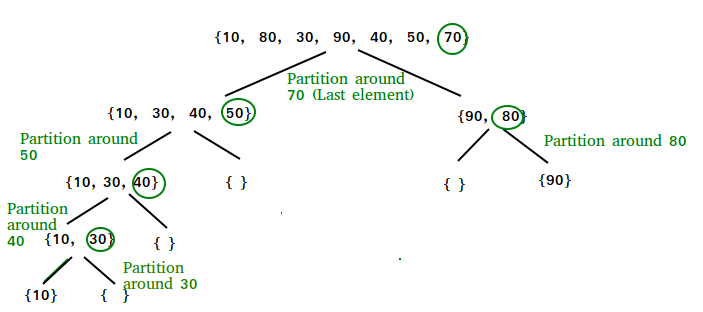
\includegraphics[width=0.8\textwidth]{figures/QuickSort2.png}
	\caption{Quicksort中的partition过程}
\end{figure}
\paragraph{Partition算法}
在quicksort中有许多种partition算法, 我采用的是一种从最左边元素开始, 跟踪
较小元素的下标i. 在循环的过程中, 如果找到一个小于x的元素,
将目前的元素和arr[i]进行交换. 否则, 不进行操作.

\subsubsection{关键函数及代码段的描述}
递归的quickSort()函数作为quicksort调用的入口, 使用尾递归调用优化来确保
$O(\log{n})$的空间复杂度.\par
partition()函数是quicksort的核心部分, 将数组元素围绕pivot按大小进行划分.\par
对函数均使用类似C++的Pseudo-Code描述.
\begin{lstlisting}[language=c++]
/**
 * Main function to perform quicksort on arr[],
 * optimized with **tail call elimination**
 */
void QuickSort::quickSort(int arr[], int l, int h) {
    while (l < h) {
        // Median of arr[]
        int pivor = arr[(l + h) / 2];

        // Partition the array around median
        int p = partition(arr, l, h, pivor);

        // If left half has less elements, recur for left half.
        // Else recur for right half.
        if (p - l < h - p) {
            quickSort(arr, l, p - 1);
            l = p + 1;
        } else {
            quickSort(arr, p + 1, h);
            h = p - 1;
        }
    }
}

// Search for x in arr[l, ..., r], then partition
// arr[] around x.
int QuickSort::partition(int arr[], int l, int r, int x) {
    int i = 0;
    // Search for x in arr[l, ..., r], if found, move it to end
    for (i = l; i < r; i++) {
        if (arr[i] == x) {
            break;
        }
    }
    swap arr[i] and arr[r];

    // Make partition
    i = l;
    for (int j = l; j <= r - 1; j++) {
        if (arr[j] <= x) {
            swap arr[i] and arr[j];
            i++;
        }
    }
    swap arr[i] and arr[r]
    return i;
}
\end{lstlisting}

\subsubsection{算法时间及空间复杂性分析}
\paragraph{空间复杂度分析}
由于quicksort主要操作都在分区partition()函数中, 而partition()函数
是原地(in-place)的, 故quicksort是原地排序算法(in-place algorithm),
不占用额外空间, 空间复杂度为O(1).\par
\textbf{然而}, 递归实现的quicksort函数会递归的两次调用自身, 在最坏
情况下会占用$O(n)$的函数调用栈上空间(与下面的时间复杂度最坏情况相同).\par
为了解决这个问题, 我使用了\textbf{尾递归优化}的方式, 改写quicksort使其
只执行一次递归调用, 即上面代码中的quickSort(), 并且, 即便在最坏的,
数组被划分为左半部分总有$n-1$个元素的情况下, quickSort()总会对较小数组部分
进行递归调用, 而对较大数组部分进行迭代调用. 这样可以保证在所有递归调用中,
也只使用$O(log{n})$的额外空间.

\paragraph{时间复杂度分析}
由于quicksort不进行比较就不会移动元素, 所以元素移动次数一定小于比较次数,
像mergesort的分析过程一样, 只需要分析比较次数即可.\par
由于快速排序是递归的过程, 可以方便地写出递推式:
\begin{align}
	C(1)       & = 0                        \nonumber \\
	C_{avg}(n) & = 2C(\frac{n}{2}) + n - 1  \nonumber \\
	C_{max}(n) & = C(1) + C(n - 1) + n - 1  \nonumber
\end{align}
令\(n=2^k\), 将式中$O(n)$项用$O(n)$代替, 得
\begin{align}
	C'(0)       & = 0                                           \nonumber \\
	C'_{avg}(k) & = 2C'_{avg}(k-1)+2^k-1                        \nonumber \\
	            & = 2C'_{avg}(0)+k\cdot 2^k - \sum_{i=0}^k 2^i  \nonumber \\
	            & = k\cdot 2^k - 2^{k+1}+1                      \nonumber \\
	            & = (k-2)\cdot 2^k + 1 \nonumber
\end{align}
故
\begin{align}
	C_{avg}(n) & = (\log_2{n}-2)\cdot n+1  \nonumber \\
	C_{max}(n) & = \sum_{i=1}^{n-1}i       \nonumber \\
	           & = \frac{n(n-1)}{2}        \nonumber \\
	           & =\frac{n^2-n}{2}          \nonumber
\end{align}
综上, quicksort的平均时间复杂度为$O(n\log n)$, 最坏时间复杂度为
$O(n^2)$.

\subsection{应用线性时间选择优化的快速排序quicksort}
\subsubsection{算法类别}
quicksort(快速排序)和mergesort一样, 也是一种\textbf{分治法}算法.
k'th smallest element in unsorted array(线性时间选择)也是一种
\textbf{分治法}算法.

\subsubsection{算法思路}
\paragraph{线性时间选择问题}
如果能在线性时间内找到一个划分基准,使得按这个基准所划分出的2个子数组
的长度都至少为原数组长度的ε倍(0<ε<1是某个正常数),那么就可以在最坏情况
下用O(n)时间完成选择任务,这是线性时间选择问题。\par
kthSmallest(arr[0, ..., n-1], k)
\begin{enumerate}
	\item 将数组划分为含最多5个元素的小数组.
	\item 将前面创建的n/5个小数组分别排序, 找到每个小数组的中位数. 这一步
	      可以选用任意的排序算法, 例如Insertion sort(插入排序). 在这一步之后,
	      产生一个数组median[], 包含所有n/5个小数组的中位数.
	\item 找到kthSmallest(median[0, ..., n/5-1], n/10).
	\item 递归的找到median[]数组的kthSmallest.
\end{enumerate}

\subsubsection{关键函数及代码段的描述}
quickSort()是对arr[]进行quicksort的入口, 用kthSmallest算法寻找中位数作为
pivot, 从而避免了退化.\par
kthSmallest()递归地寻找arr[]中的k'th最小元素, 最坏情况下只使用线性时间.\par
findMedian()使用插入排序寻找数组的中位数. 在本算法中只对大小为5的数组使用.\par
partition()对数组arr[]根据pivot x进行分区.\par
函数均使用类似C++的Pseudo-Code进行描述.
\begin{lstlisting}[language=c++]
/**
 * Main function to perform quicksort on arr[],
 * optimized with **tail call elimination**
 */
void QuickSort::quickSort(int arr[], int l, int h) {
    while (l < h) {
        int n = size of current subarray;

        int med = find median of arr[] using kthSmallest();

        // Partition the array around median
        int p = partition(arr, l, h, med);

        // tail recursive call elimination
        if (p - l < h - p) {
            quickSort(arr, l, p - 1);
            l = p + 1;
        } else {
            quickSort(arr, p + 1, h);
            h = p - 1;
        }
    }
}

/**
 * recursively find kth smallest element in arr[]
 * in worst linear time
 */
int QuickSort::kthSmallest(int arr[], int l, int r, int k) {
    // Indeces range from 1.
    if (k is smaller than number of elements in array) {
        int n = number of elements in arr.

        int i = 0;
        Divide arr[] in groups of size 5, then store median
        of each group in median[] array with findMedian()

        // Recursively find median of all medians.
        int medOfMed =
            (i == 1) ? median[0] : kthSmallest(median, 0, i - 1, i / 2);

        int pos = partition(arr, l, r, medOfMed);

        if (pos - l == k - 1) {
            return arr[pos];
        } else if (pos - l > k - 1) {
            return kthSmallest(arr, l, pos - 1, k);
        }

        return kthSmallest(arr, pos + 1, r, k - (pos - l) - 1);
    }

    // If k is more than number of elements in arr[]
    return INT_MAX;
}

// A simple function to find median of arr[]. This is called
// only for an array of size 5 in this program, thus has an
// time complexity of O(1).
int QuickSort::findMedian(int arr[], int n) {
  	Simple insertion sort on arr[];

    return arr[n / 2];
}

// Search for x in arr[l, ..., r], then partition
// arr[] around x.
int QuickSort::partition(int arr[], int l, int r, int x) {
    int i = 0;
    Search for x in arr[l, ..., r];
    if (found) {
			swap arr[i] and arr[r];
    }

    // Make partition
    i = l;
    for (int j = l; j <= r - 1; j++) {
        if (arr[j] <= x) {
            swap arr[i] and arr[j];
            i++;
        }
    }
  	swap arr[i] and arr[r];
    return i;
}
\end{lstlisting}

\subsubsection{算法时间及空间复杂性分析}
\paragraph{空间复杂度分析}
由于与上面的quicksort采用了相同的尾递归调用优化, 同样有$O(log{n})$的
考虑函数调用栈上空间占用的空间复杂度.

\paragraph{时间复杂度分析}
TODO

\section{实验结果}
本节应至少包括三方面:
1.程序执行环境及运行方式;
2.程序输入及输出格式;
3.程序执行示例。此处应添加一至多个程序执行示例,以反应在不同的初始条件下算法的正确性。
\begin{enumerate}
\item 词法分析程序的作用:
  \begin{enumerate}
  \item 扫描源程序字符流;
  \item 按照源语言的词法规则识别出各类单词符号;
  \item 产生用于语法分析的记号序列;
  \item 词法检查;
  \item 创建符号表, 将识别出来的标识符放入符号表中;
  \item 跳过源程序中的注释和空格等, 把错误信息和源代码联系起来;
  \end{enumerate}
\item 源程序代词类别:
  \begin{enumerate}
    \item 关键字;
    \item 用户定义变量标识符;
    \item 数字, 字符和字符串常量;
    \item 运算符;
    \item 分隔符;
  \end{enumerate}
\item 设计思路:
  利用有限状态自动机模型, 将整个源代码分析的过程转化为不同状态之间的转移, 在画好
  状态转移图之后, 借用C++的switch语句或if/else语句将状态转移图描述出来. 此外, 
  实现好读取源代码, 缓冲区, 以及输出分析结果, 和将常量和变量名插入到符号表的功能.
\item 伪代码描述:
\begin{lstlisting}
// Initializing...
while(End of source file not reached) {
  ch = getchar();
  switch(ch) {
    determine state based on the input char
    case 0:
    ...
  }
  switch(State) {
    // Limited state machine process
    case 0:
      // state 0 process
    case 1:
      // state 1 process
    ...
  }
}
\end{lstlisting}
\end{enumerate}

\section{实验总结}
\label{ssub:实验心得}
通过这次实验, 我亲手实现并测试了读者优先进程调度和写者优先进程调度, 对信号量机制
来控制并行进程对关键区的访问有了更深刻的认识.

在构建和管理项目的工具方面, 使用了make工具, 方便的实现了
对程序的构建和测试; 此外, 对于文档, 也使用了make工具作为管理,
很大程度上方便了实验报告修改后的再次编译. 在实验报告编写方面,
练习了latex的使用, 对latex语法和使用更加熟悉.\par

但是, 由于时间限制, 没有来得及进行更多更详细的测试, 例如, 从10\%读者到90\%读者每
个进行2000个进程运行的读者优先和写者优先策略测试等. 但是即便如此, 也已经有了丰富的收获.

总的来说, 这次实验在信号量机制进程调度之内及之外都学到了许多知识, 收获颇丰.
% subsection 实验心得 (end)

\section{算法源代码}
在此处粘贴算法的源代码,注意应对关键的变量、函数及代码段加以注释。
\lstinputlisting{../mergesort/mergesort.cpp}

\section{附录}
代码仓库: \href
{https://github.com/Micuks/code/tree/master/oslab/}
{OSLab}

% \bibliographystyle{ieeetrans}
% \bibliography{Assignment_Ref}

\end{document}
